\documentclass[a4paper]{article}
\usepackage{vntex}
%\usepackage[english,vietnam]{babel}
%\usepackage[utf8]{inputenc}

%\usepackage[utf8]{inputenc}
%\usepackage[francais]{babel}
\usepackage{a4wide,amssymb,epsfig,latexsym,multicol,array,hhline,fancyhdr}
\usepackage{booktabs}
\usepackage{amsmath}
\usepackage{lastpage}
\usepackage[lined,boxed,commentsnumbered]{algorithm2e}
\usepackage{enumerate}
\usepackage{color}
\usepackage{graphicx}							% Standard graphics package
\usepackage{array}
\usepackage{tabularx, caption}
\usepackage{multirow}
\usepackage[framemethod=tikz]{mdframed}% For highlighting paragraph
\usepackage{adjustbox}
%\backgrounds
\usepackage{multicol}
\usepackage{rotating}
\usepackage{graphics}
\usepackage{geometry}
\usepackage{setspace}
\usepackage{epsfig}
\usepackage{tikz}
\usepackage{listings}
\usetikzlibrary{arrows,snakes,backgrounds}
\usepackage{hyperref}
\hypersetup{urlcolor=blue,linkcolor=black,citecolor=black,colorlinks=true} 

% Chỉ định encoding UTF-8 cho gói listings
\lstset{
    inputencoding=utf8,
    extendedchars=true,
    literate=%
    {á}{{\'a}}1
    {à}{{\`a}}1
    {ả}{{\~a}}1
    {ã}{{\~a}}1
    {ạ}{{\d{a}}}1
    {â}{{\^a}}1
    {ấ}{{\'a}}1
    {ầ}{{\`a}}1
    {ẩ}{{\~a}}1
    {ẫ}{{\~a}}1
    {ậ}{{\d{a}}}1
    {ă}{{\u{a}}}1
    {ắ}{{\'a}}1
    {ằ}{{\`a}}1
    {ẳ}{{\~a}}1
    {ẵ}{{\~a}}1
    {ặ}{{\d{a}}}1
    {ó}{{\'o}}1
    {ò}{{\`o}}1
    {ỏ}{{\~o}}1
    {õ}{{\~o}}1
    {ọ}{{\d{o}}}1
    {ô}{{\^o}}1
    {ố}{{\'o}}1
    {ồ}{{\`o}}1
    {ổ}{{\~o}}1
    {ỗ}{{\~o}}1
    {ộ}{{\d{o}}}1
    {ơ}{{\^{o}}}1
    {ớ}{{\'{o}}}1
    {ờ}{{\`{o}}}1
    {ở}{{\~{o}}}1
    {ỡ}{{\~{o}}}1
    {ợ}{{\d{o}}}1
    {é}{{\'e}}1
    {è}{{\`e}}1
    {ẻ}{{\~e}}1
    {ẽ}{{\~e}}1
    {ẹ}{{\d{e}}}1
    {ê}{{\^e}}1
    {ế}{{\'e}}1
    {ề}{{\`e}}1
    {ể}{{\~e}}1
    {ễ}{{\~e}}1
    {ệ}{{\d{e}}}1
    {ú}{{\'u}}1
    {ù}{{\`u}}1
    {ủ}{{\~u}}1
    {ũ}{{\~u}}1
    {ụ}{{\d{u}}}1
    {ư}{{\^{u}}}1
    {ứ}{{\'{u}}}1
    {ừ}{{\`{u}}}1
    {ử}{{\~{u}}}1
    {ữ}{{\~{u}}}1
    {ự}{{\d{u}}}1
    {í}{{\'i}}1
    {ì}{{\`i}}1
    {ỉ}{{\~i}}1
    {ĩ}{{\~i}}1
    {ị}{{\d{i}}}1
    {ý}{{\'y}}1
    {ỳ}{{\`y}}1
    {ỷ}{{\~y}}1
    {ỹ}{{\~y}}1
    {ỵ}{{\d{y}}}1
    {Á}{{\'A}}1
    {À}{{\`A}}1
    {Ả}{{\~A}}1
    {Ã}{{\~A}}1
    {Ạ}{{\d{A}}}1
    {Â}{{\^A}}1
    {Ấ}{{\'A}}1
    {Ầ}{{\`A}}1
    {Ẩ}{{\~A}}1
    {Ẫ}{{\~A}}1
    {Ậ}{{\d{A}}}1
    {Ă}{{\u{A}}}1
    {Ắ}{{\'A}}1
    {Ằ}{{\`A}}1
    {Ẳ}{{\~A}}1
    {Ẵ}{{\~A}}1
    {Ặ}{{\d{A}}}1
    {Ó}{{\'O}}1
    {Ò}{{\`O}}1
    {Ỏ}{{\~O}}1
    {Õ}{{\~O}}1
    {Ọ}{{\d{O}}}1
    {Ô}{{\^O}}1
    {Ố}{{\'O}}1
    {Ồ}{{\`O}}1
    {Ổ}{{\~O}}1
    {Ỗ}{{\~O}}1
    {Ộ}{{\d{O}}}1
    {Ơ}{{\^{O}}}1
    {Ớ}{{\'{O}}}1
    {Ờ}{{\`{O}}}1
    {Ở}{{\~{O}}}1
    {Ỡ}{{\~{O}}}1
    {Ợ}{{\d{O}}}1
    {É}{{\'E}}1
    {È}{{\`E}}1
    {Ẻ}{{\~E}}1
    {Ẽ}{{\~E}}1
    {Ẹ}{{\d{E}}}1
    {Ê}{{\^E}}1
    {Ế}{{\'E}}1
    {Ề}{{\`E}}1
    {Ể}{{\~E}}1
    {Ễ}{{\~E}}1
    {Ệ}{{\d{E}}}1
    {Ú}{{\'U}}1
    {Ù}{{\`U}}1
    {Ủ}{{\~U}}1
    {Ũ}{{\~U}}1
    {Ụ}{{\d{U}}}1
    {Ư}{{\^{U}}}1
    {Ứ}{{\'{U}}}1
    {Ừ}{{\`{U}}}1
    {Ử}{{\~{U}}}1
    {Ữ}{{\~{U}}}1
    {Ự}{{\d{U}}}1
    {Í}{{\'I}}1
    {Ì}{{\`I}}1
    {Ỉ}{{\~I}}1
    {Ĩ}{{\~I}}1
    {Ị}{{\d{I}}}1
    {Ý}{{\'Y}}1
    {Ỳ}{{\`Y}}1
    {Ỷ}{{\~Y}}1
    {Ỹ}{{\~Y}}1
    {Ỵ}{{\d{Y}}}1
}

%\usepackage{pstcol} 								% PSTricks with the standard color package



\newtheorem{theorem}{{\bf Định lý}}
\newtheorem{property}{{\bf Tính chất}}
\newtheorem{proposition}{{\bf Mệnh đề}}
\newtheorem{corollary}[proposition]{{\bf Hệ quả}}
\newtheorem{lemma}[proposition]{{\bf Bổ đề}}

\everymath{\color{blue}}
%\usepackage{fancyhdr}
\setlength{\headheight}{40pt}
\pagestyle{fancy}
\fancyhead{} % clear all header fields
\fancyhead[L]{
 \begin{tabular}{rl}
    \begin{picture}(25,15)(0,0)
    \put(0,-8){
\includegraphics[width=8mm, height=8mm]{logoITSGUsmall.png}}
    %\put(0,-8){\epsfig{width=10mm,figure=hcmut.eps}}
   \end{picture}&
	%\includegraphics[width=8mm, height=8mm]{hcmut.png} & %
	\begin{tabular}{l}
		\textbf{\bf \ttfamily Trường Đại học Sài Gòn}\\
		\textbf{\bf \ttfamily Khoa Công Nghệ Thông Tin}
	\end{tabular} 	
 \end{tabular}
}
\fancyhead[R]{
	\begin{tabular}{l}
		\tiny \bf \\
		\tiny \bf 
	\end{tabular}  }
\fancyfoot{} % clear all footer fields
\fancyfoot[L]{\scriptsize \ttfamily Bài tập lớn môn Phát triển phần mềm mã nguồn mở - Niên khóa 2023-2024}
\fancyfoot[R]{\scriptsize \ttfamily Trang {\thepage}/\pageref{LastPage}}
\renewcommand{\headrulewidth}{0.3pt}
\renewcommand{\footrulewidth}{0.3pt}


%%%
\setcounter{secnumdepth}{4}
\setcounter{tocdepth}{3}
\makeatletter
\newcounter {subsubsubsection}[subsubsection]
\renewcommand\thesubsubsubsection{\thesubsubsection .\@alph\c@subsubsubsection}
\newcommand\subsubsubsection{\@startsection{subsubsubsection}{4}{\z@}%
                                     {-3.25ex\@plus -1ex \@minus -.2ex}%
                                     {1.5ex \@plus .2ex}%
                                     {\normalfont\normalsize\bfseries}}
\newcommand*\l@subsubsubsection{\@dottedtocline{3}{10.0em}{4.1em}}
\newcommand*{\subsubsubsectionmark}[1]{}
\makeatother

\definecolor{dkgreen}{rgb}{0,0.6,0}
\definecolor{gray}{rgb}{0.5,0.5,0.5}
\definecolor{mauve}{rgb}{0.58,0,0.82}

\lstset{frame=tb,
	language=Matlab,
	aboveskip=3mm,
	belowskip=3mm,
	showstringspaces=false,
	columns=flexible,
	basicstyle={\small\ttfamily},
	numbers=none,
	numberstyle=\tiny\color{gray},
	keywordstyle=\color{blue},
	commentstyle=\color{dkgreen},
	stringstyle=\color{mauve},
	breaklines=true,
	breakatwhitespace=true,
	tabsize=3,
	numbers=left,
	stepnumber=1,
	numbersep=1pt,    
	firstnumber=1,
	numberfirstline=true
}

\begin{document}

\begin{titlepage}
\begin{center}
TRƯỜNG ĐẠI HỌC SÀI GÒN \\
KHOA CÔNG NGHỆ THÔNG TIN
\end{center}
\vspace{1cm}

\begin{figure}[h!]
\begin{center}

\includegraphics[width=8cm]{logoITSGU.png}
\end{center}
\end{figure}

\vspace{0.5cm}


\begin{center}
\begin{tabular}{c}
	\multicolumn{1}{l}{\textbf{{\Large PHÁT TRIỂN PHẦN MỀM MÃ NGUỒN MỞ}}}\\
	~~\\
	\hline
	\\
	\multicolumn{1}{l}{\textbf{{\Large Xây dựng game bằng Pygame}}}\\
	\\
	
	\textbf{{\Huge Pacman Game with Socket}}\\
	\\
	\hline
\end{tabular}
\end{center}


\begin{table}[h]
\begin{tabular}{rrl}
\hspace{8 cm} & GVHD: &Từ Lãng Phiêu\\
& SV: & Đỗ Lê Huy - 3120410201\\
& & Nguyễn Thị Bích Ngọc - 3120410348 \\
& & Phan Thị Kim Phụng - 3120410416 \\
% & & SV3 - MSSV \\
% & & SV4 - MSSV\\
\end{tabular}
\vspace{1.2 cm}
\end{table}

\begin{center}

{\footnotesize TP. HỒ CHÍ MINH, THÁNG 05/2024}
\end{center}


\end{titlepage}


\thispagestyle{empty}

\newpage
\tableofcontents
\newpage

%%%%%%%%%%%%%%%%%%%%%%%%%%%%%%%%%


%%%%%%%%%%%%%%%%%%%%%%%%%%%%%%%%%
\section{Giới Thiệu}

Trong phần này, chúng tôi sẽ giới thiệu chung về đồ án và trò chơi Pacman đa người chơi sử dụng Socket.

\subsection{Giới Thiệu Chung}

Trò chơi Pacman là một trong những trò chơi kinh điển trong lịch sử game và luôn là một trong những lựa chọn phổ biến của người chơi. Với mục tiêu mang lại trải nghiệm mới mẻ và thú vị cho người chơi, chúng tôi đã quyết định phát triển một phiên bản đa người chơi của trò chơi này, sử dụng công nghệ Socket để tạo ra một môi trường chơi trực tuyến.

\subsection{Mô Tả về Đề Tài}

Đồ án này tập trung vào việc phát triển trò chơi Pacman đa người chơi, nơi mà người chơi có thể tham gia vào trò chơi cùng nhau thông qua mạng máy tính. Trò chơi sẽ bao gồm các tính năng cơ bản của trò chơi Pacman như điều khiển nhân vật, ăn viên gạch và tránh ma, cùng với tính năng đa người chơi cho phép nhiều người cùng tham gia vào cùng một trò chơi và tương tác với nhau tiêu diệt lẫn nhau để giành lấy số điểm của người khác.




\newpage
%%%%%%%%%%%%%%%%%%%%%%%%%%%%%%%%%
\section{Phân Tích Yêu Cầu}

Trước khi bắt đầu phát triển, việc phân tích yêu cầu là bước quan trọng để hiểu rõ các tính năng và chức năng mà trò chơi Pacman đa người chơi sử dụng Socket cần phải có. Phân tích yêu cầu cung cấp một cơ sở cho việc thiết kế và hiện thực của trò chơi, đồng thời giúp định rõ phạm vi và mục tiêu của dự án.

\subsection{Yêu Cầu Chức Năng}

Trò chơi Pacman đa người chơi sẽ có một số tính năng chức năng cơ bản sau:

\begin{itemize}
    \item \textbf{Điều Khiển Nhân Vật:} Người chơi có thể điều khiển nhân vật Pacman để di chuyển trong mê cung và ăn các viên gạch.
    \item \textbf{Tránh Ma:} Nhân vật Pacman phải tránh xa các ma trong mê cung, nếu bị ma tấn công sẽ mất mạng.
    \item \textbf{Ăn Viên Gạch:} Mục tiêu của người chơi là ăn càng nhiều viên gạch càng tốt.
    \item \textbf{Tránh sự tấn công của người chơi khác:} Khi người chơi khác ăn viên gạch lớn bạn sẽ bị rơi vào trạng thái nguy hiểm và có thể bị người chơi khác tấn công gây mất một nửa điểm số.
    \item \textbf{Giao Diện Người Dùng:} Trò chơi cần có một giao diện người dùng đơn giản, hiển thị điểm số, màn hình mê cung và hộp thoại tin nhắn với người chơi khác.
    \item \textbf{Chơi Đa Người Chơi:} Tính năng chơi đa người chơi cho phép nhiều người chơi tham gia vào cùng một trò chơi Pacman và có thể trò chuyện với nhau và tương tác với nhau trong trò chơi.
\end{itemize}

\subsection{Yêu Cầu Phi Chức Năng}

Ngoài các tính năng chức năng cơ bản, trò chơi cũng cần phải đáp ứng các yêu cầu phi chức năng sau:

\begin{itemize}
    \item \textbf{Độ Ổn Định:} Trò chơi cần phải ổn định và không gặp lỗi khi chơi.
    \item \textbf{Hiệu Suất:} Trò chơi cần phải chạy mượt mà và không gây ra hiện tượng giật lag.
\end{itemize}

Việc hiểu rõ các yêu cầu chức năng và phi chức năng này là quan trọng để đảm bảo rằng trò chơi Pacman đa người chơi sẽ đáp ứng được mong đợi của người chơi và đáp ứng được tiêu chuẩn chất lượng.


\newpage
%%%%%%%%%%%%%%%%%%%%%%%%%%%%%%%%%
\section{Thiết Kế}

Trong phần này, chúng tôi sẽ mô tả về cách mà trò chơi Pacman đa người chơi sử dụng Socket được thiết kế và tổ chức.

\subsection{Sơ Đồ Hoạt Động}

Sơ đồ luồng hoạt động chính dưới đây mô tả cấu trúc của trò chơi.

\begin{figure}[h!]
    \centering
    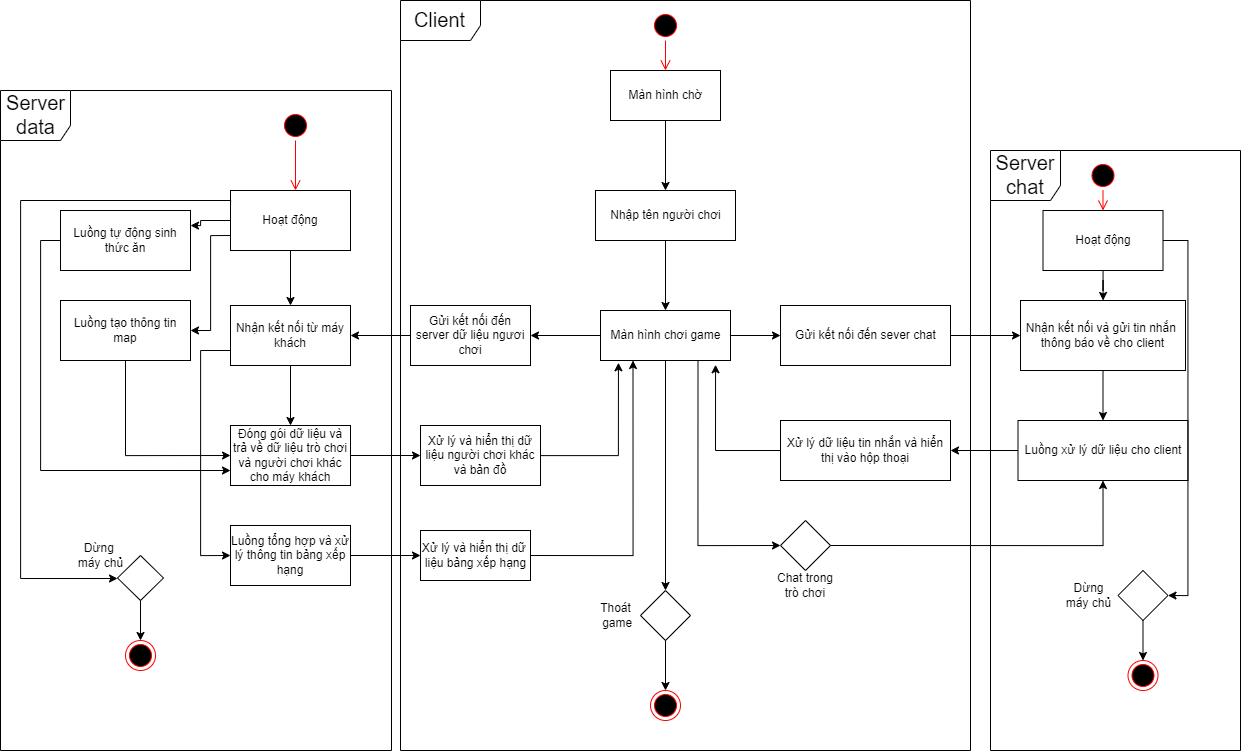
\includegraphics[width=1\linewidth]{luongHoatDongChinh.png}
    \caption{Luồng hoạt động chính của chương trình.}
\end{figure}

\subsection{Giao Diện Người Dùng}

Giao diện người dùng của trò chơi bao gồm các thành phần sau:
\newpage
\subsubsection{Màn hình chờ: Hiển thị ô nhập tên người chơi và tên của trò chơi.}
\begin{figure}[h!]
    \centering
    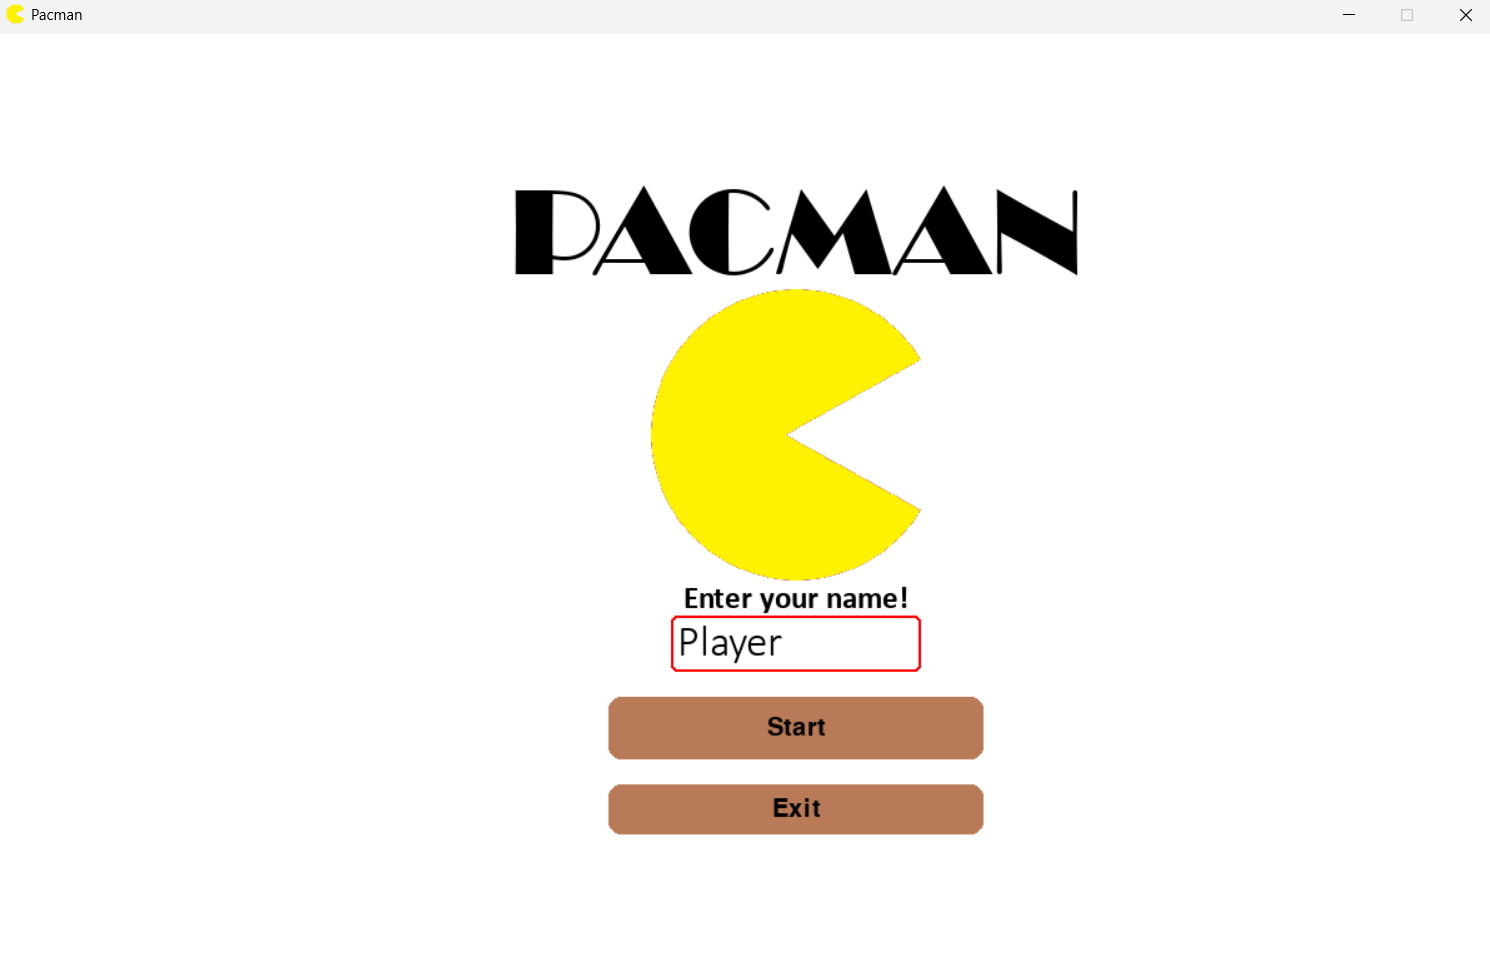
\includegraphics[width=1\linewidth]{manHinhCho.png}
    \caption{Màn hình chờ}
\end{figure}

\newpage
\subsubsection{Màn hình chơi: Hiển thị trạng thái của trò chơi và các đối tượng.}
\begin{figure}[h!]
    \centering
    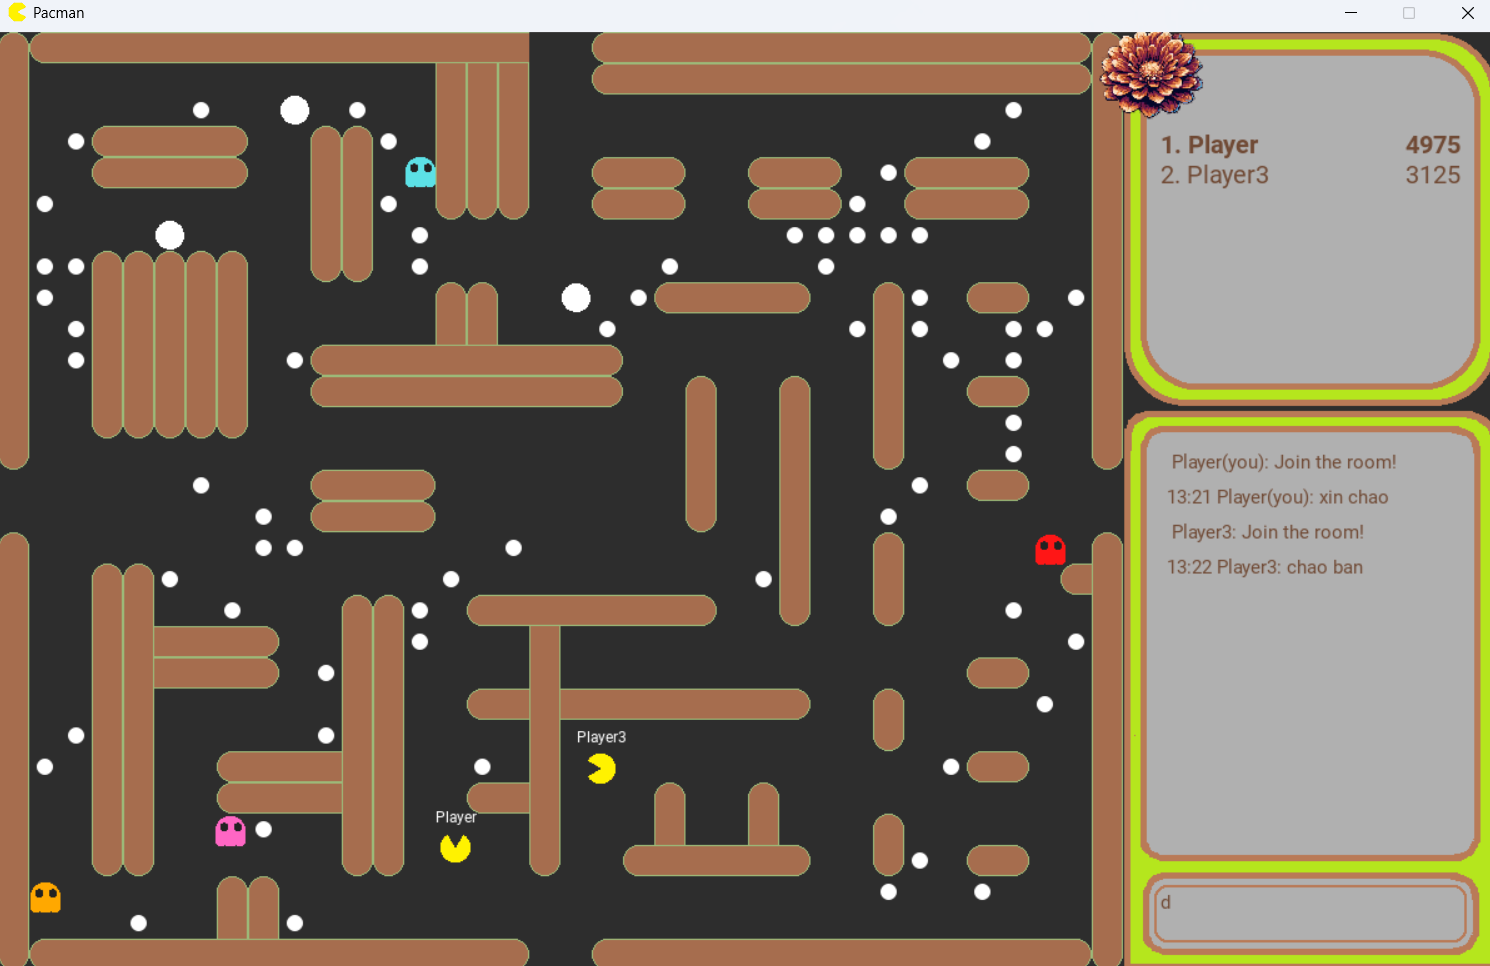
\includegraphics[width=1\linewidth]{manHinhTroChoi.png}
    \caption{Màn hình chính của trò chơi}
\end{figure}

\newpage
\subsubsection{Bảng điểm: Hiển thị xếp hạng của người chơi.}
\begin{figure}[h!]
    \centering
    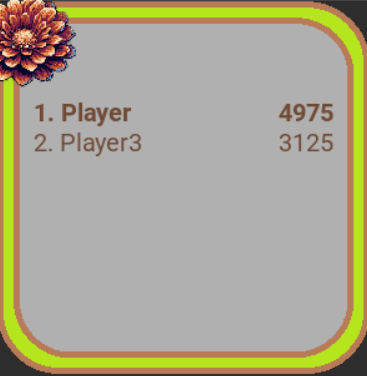
\includegraphics[width=1\linewidth]{score.png}
    \caption{Khung bảng điểm}
\end{figure}

\newpage
\subsubsection{Khung trò chuyện: Hiển thị dữ liệu trò chuyện giữa các người chơi.}
\begin{figure}[h!]
    \centering
    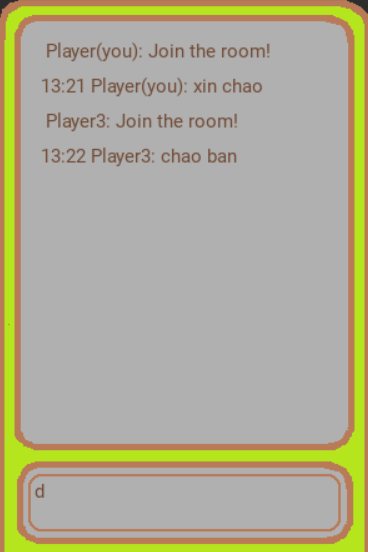
\includegraphics[valign=20cm, height=18cm]{messageBox.png}
    \caption{Khung chat}
\end{figure}


\newpage
\subsection{Xử Lý Logic và Luật Chơi}

Trong trò chơi Pacman, logic và luật chơi được xử lý như sau:

\begin{itemize}
    \item \textbf{Di Chuyển Nhân Vật:} Người chơi có thể điều khiển nhân vật Pacman bằng các phím A, S, W, D tương ứng với trái, xuống, lên, phải. Logic xử lý việc di chuyển của Pacman cũng như hạn chế các hành động không hợp lệ.
    \item \textbf{Ăn Gạch:} Khi Pacman đi qua một viên gạch, viên gạch sẽ biến mất và người chơi sẽ được điểm số tương ứng.
    \item \textbf{Tránh Ma:} Pacman phải tránh xa các con ma để không bị chúng tấn công. Nếu Pacman bị tấn công, số điểm của người chơi sẽ giảm.
    \item \textbf{Điểm Số:} Điểm số của người chơi giảm mỗi khi Pacman bị tấn công bởi ma hoặc người chơi khác. Điểm số tăng mỗi khi Pacman ăn được một viên gạch hoặc hạ gục một người chơi khác
\end{itemize}

\subsection{Cơ Chế Tương Tác Mạng}

Trò chơi sử dụng Socket để tương tác mạng giữa máy chủ và người chơi.
\begin{itemize}
    \item \textbf{Dữ liệu nhân vật và bản đồ:} Sử dụng socket dựa trên giao thúc UDP để gửi dữ liệu nhắm đạt được tốc độ truyền tải cao hơn.
    \item \textbf{Dữ liệu trò chuyện:} Sử dụng socket dựa trên giao thức TCP để gửi dữ liệu nhắm đảm bảo an toàn cho dữ liệu được gửi đi.
\end{itemize}
\newpage
%%%%%%%%%%%%%%%%%%%%%%%%%%%%%%%%%
\section{Mã Nguồn}

Dưới đây là các đoạn mã nguồn quan trọng trong quá trình triển khai trò chơi Pacman:

\subsection{Mã Python phía client}

\subsubsection{Hàm nhận dữ liệu từ server}

\begin{lstlisting}[language=Python]
def receive_data():
    global red_ghost_x, red_ghost_y, red_ghost_direction, red_ghost_dead, red_dead_time_count, red_dead_time_default, \
        blue_ghost_x, blue_ghost_y, blue_ghost_direction, blue_ghost_dead, blue_dead_time_count, \
        blue_dead_time_default, orange_ghost_x, orange_ghost_y, orange_ghost_direction, orange_ghost_dead, \
        orange_dead_time_count, orange_dead_time_default, pink_ghost_x, pink_ghost_y, pink_ghost_direction, \
        pink_ghost_dead, pink_dead_time_count, pink_dead_time_default, ghost_speeds, map_level, player_dead, \
        player_x, player_y, ghost_is_slow, other_player_data, total_score, data_score_table, player_slowing, \
        player_slowing_clock
    while game_running:
        try:
            response, server_address = client_socket.recvfrom(4096)
            data = json.loads(response.decode())

            data_map = data.get("map")
            if data_map is not None:
                # data map
                map_level = data_map
                # data ghost
                data_ghost = data["ghost"]
                ghost_speeds = data_ghost[24]
                ghost_is_slow = data_ghost[25]
                # data red ghost
                red_ghost_x = data_ghost[0]
                red_ghost_y = data_ghost[1]
                red_ghost_direction = data_ghost[2]
                red_ghost_dead = data_ghost[3]
                red_dead_time_count = data_ghost[4]
                red_dead_time_default = data_ghost[5]
                # data blue ghost
                blue_ghost_x = data_ghost[6]
                blue_ghost_y = data_ghost[7]
                blue_ghost_direction = data_ghost[8]
                blue_ghost_dead = data_ghost[9]
                blue_dead_time_count = data_ghost[10]
                blue_dead_time_default = data_ghost[11]
                # data orange ghost
                orange_ghost_x = data_ghost[12]
                orange_ghost_y = data_ghost[13]
                orange_ghost_direction = data_ghost[14]
                orange_ghost_dead = data_ghost[15]
                orange_dead_time_count = data_ghost[16]
                orange_dead_time_default = data_ghost[17]
                # data pink ghost
                pink_ghost_x = data_ghost[18]
                pink_ghost_y = data_ghost[19]
                pink_ghost_direction = data_ghost[20]
                pink_ghost_dead = data_ghost[21]
                pink_dead_time_count = data_ghost[22]
                pink_dead_time_default = data_ghost[23]

            data_you = data.get("you")
            if data_you is not None:
                total_score = data_you[6]
                if data_you[4]:
                    player_dead = True
                    player_x = data_you[1]
                    player_y = data_you[2]
                if data_you[9]:
                    if player_slowing:
                        player_slowing_clock += player_slowing_clock_default
                    else:
                        player_slowing = True
                else:
                    player_slowing = False

            data_other_player = data.get("otherPlayer")
            if data_other_player is not None:
                other_player_data[data_other_player[0]] = data_other_player

            data_score = data.get("score_table")
            if data_score is not None:
                data_score_table = data_score

        except:
            pass


receive_data_thread = threading.Thread(target=receive_data)
receive_data_thread.start()
\end{lstlisting}
Dùng một luồng riêng để nhận dữ liệu từ máy chủ và đặt chúng cho các thuộc tính trong client để phục vụ cho việc hiển thị.

\subsubsection{Hàm gửi dữ liệu của người chơi lên máy chủ}
\begin{lstlisting}[language=Python]
def send_data():
    player_dead_default = False
    json_data = json.dumps(
        [nick_name, player_x, player_y, player_direction, player_dead_default, is_flickering_player, total_score,
         is_visible_player, loop_count_player, player_slowing
         ]
    )
    # gửi dữ liệu lên server
    client_socket.sendto(json_data.encode(), server_address)
\end{lstlisting}
Việc gửi dữ liệu của người chơi lên máy chủ được thực hiện trong vòng lặp chính khi game chạy.

\subsubsection{Hàm gửi dữ liệu tin nhắn lên máy chủ}
\begin{lstlisting}[language=Python]
def send_message(message):
    # gửi dữ liệu
    client_message.send(json.dumps(message).encode())
\end{lstlisting}
Hàm này được gọi khi người dùng quyết định gửi tin nhắn của mình đi.


\subsubsection{Hàm nhận dữ liệu tin nhắn từ máy chủ}
\begin{lstlisting}[language=Python]
def receive_message_game_main():
    while game_running:
        try:
            # nhận dữ liệu từ server
            data = client_message.recv(1024).decode()
            json_data = json.loads(data)
            if json_data[0] == "LEFT_ROOM":
                other_player_data.pop(json_data[1])
                json_data[0] = ""
            message_box.add_message(json_data)
        except:
            pass

receive_thread_message = threading.Thread(target=receive_message_game_main)
receive_thread_message.start()
\end{lstlisting}
Việc nhận tin nhắn từ máy chủ được thực thi trên một luồng riêng biệt nhằm đảm bảo không bị ngắt quãng luồng chính của trò chơi.


\newpage
\subsubsection{Hàm xử lý va chạm người chơi với tường}
\begin{lstlisting}[language=Python]
def check_position(location_x, location_y):
    turns = [False, False, False, False]  # Right, Left, Up, Down
    # Left
    if map_level[location_y // 25][(location_x - speed_player) // 25] < 3 \
            and map_level[(location_y + HEIGHT_PACMAN) // 25][(location_x - speed_player) // 25] < 3:
        turns[1] = True
    # Right
    if map_level[location_y // 25][(location_x + WIDTH_PACMAN + speed_player) // 25] < 3 \
            and map_level[(location_y + HEIGHT_PACMAN) // 25][(location_x + WIDTH_PACMAN) // 25] < 3:
        turns[0] = True
    # Down
    if map_level[(location_y + HEIGHT_PACMAN + speed_player) // 25][location_x // 25] < 3 \
            and map_level[(location_y + HEIGHT_PACMAN + speed_player) // 25][(location_x + WIDTH_PACMAN) // 25] < 3:
        turns[3] = True
    # Up
    if map_level[(location_y - speed_player) // 25][location_x // 25] < 3 \
            and map_level[(location_y - speed_player) // 25][(location_x + WIDTH_PACMAN) // 25] < 3:
        turns[2] = True
    return turns
\end{lstlisting}
Việc kiểm tra và chạm trường được thức hiện dựa trên việc kiểm tra khả năng có thế di chuyển 4 hướng của người chơi để di chuyển người chơi trong bước tiếp theo. Lấy vị trí hiện tại của người chơi và tính toán để đưa về số dòng và cột trong ma trận bản đồ để biết được ô tiếp theo người chơi có thể di chuyển đến hay không. Một ví dụ về các kiểm tra di chuyển người chơi ở hình bên dưới.

\newpage
\begin{figure}[h!]
    \centering
    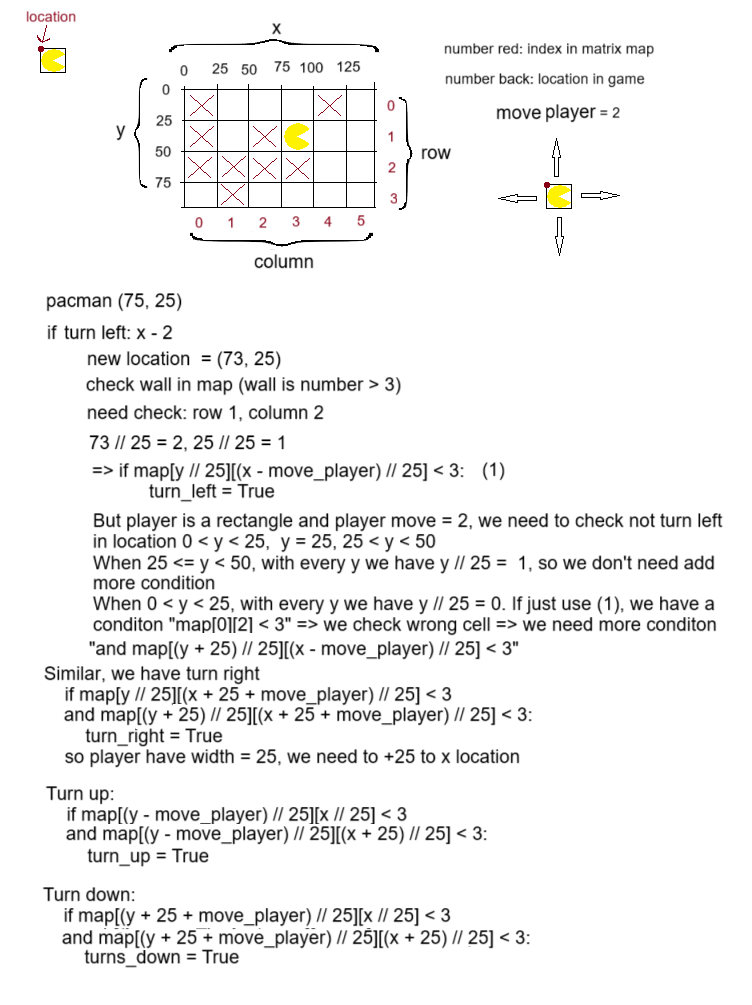
\includegraphics[height=18cm]{check_collision_wall.png}
    \caption{Kiểm tra hướng di chuyển của người chơi}
\end{figure}



\newpage
\subsubsection{Luồng chính của client}

\begin{lstlisting}[language=Python]
while game_running:
    try:
        # set fps
        timer.tick(fps)

        # event
        for event in pygame.event.get():
            if event.type == pygame.QUIT:
                game_running = False
            if len(input_text_box_message.text) < limit_text_length_message + 1:
                input_text_box_message.handle_event(event, handle_enter_input_box_message)
            message_box.handle_event(event)

        # if player dead
        if player_dead and not is_flickering_player:
            is_flickering_player = True

        # thoi gian nhap nhay pacman
        if is_flickering_player and player_flicker_time_count > 0:
            player_flicker_time_count -= 1
            # nhấp nháy pacman
            if count_flicker_player < 10:
                count_flicker_player += 1
                is_visible_player = False
            elif count_flicker_player < 20:
                count_flicker_player += 1
                is_visible_player = True
            else:
                count_flicker_player = 0
        else:
            is_flickering_player = False
            player_dead = False
            is_visible_player = True
            player_flicker_time_count = player_flicker_time_default

        # thoi gian player slowing
        if player_slowing and player_slowing_clock > 0:
            player_slowing_clock -= 1
        else:
            player_slowing = False
            player_slowing_clock = player_slowing_clock_default

        # send data to server
        send_data()

        # flicker big food 
        if loop_flicker_food_clock < 50:
            loop_flicker_food_clock += 1
            # thời gian ẩn
            if loop_flicker_food_clock > 10:
                flicker_food = False
        else:
            loop_flicker_food_clock = 0
            flicker_food = True

        # co ham pacman
        if loop_count_player < 19:
            loop_count_player += 1
        else:
            loop_count_player = 0

        # set background
        screen.fill(background_color)

        # turn alowed pacman
        turns_allowed = check_position(player_x, player_y)

        #  move to gate
        if player_x > WIDTH_PLAYING - 30:
            player_x = 15
        if player_x < 5:
            player_x = WIDTH_PLAYING - 30
        if player_y > HEIGHT_PLAYING - 30:
            player_y = 5
        if player_y < 5:
            player_y = HEIGHT_PLAYING - 30

        # call method draw
        # wall
        draw_map()

        # pacman
        draw_player(is_visible_player, loop_count_player, player_x, player_y, player_direction, nick_name,
                    player_slowing)

        draw_other_player()

        # red ghost
        red_ghost = Ghost(red_ghost_x, red_ghost_y, ghost_speeds[0], red_ghost_image, red_ghost_direction, red_ghost_dead)
        flicker_red_ghost_clock = red_ghost.draw(flicker_red_ghost_clock)

        # blue ghost
        blue_ghost = Ghost(blue_ghost_x, blue_ghost_y, ghost_speeds[1], blue_ghost_image, blue_ghost_direction,
                           blue_ghost_dead)
        flicker_blue_ghost_clock = blue_ghost.draw(flicker_blue_ghost_clock)

        # pink ghost
        pink_ghost = Ghost(pink_ghost_x, pink_ghost_y, ghost_speeds[2], pink_ghost_image, pink_ghost_direction,
                           pink_ghost_dead)
        flicker_pink_ghost_clock = pink_ghost.draw(flicker_pink_ghost_clock)

        # orange ghost
        orange_ghost = Ghost(orange_ghost_x, orange_ghost_y, ghost_speeds[3], orange_ghost_image, orange_ghost_direction,
                             orange_ghost_dead)
        flicker_orange_ghost_clock = orange_ghost.draw(flicker_orange_ghost_clock)

        # score
        draw_score(data_score_table)

        # message
        draw_message_box()

        # move player
        key_pressed = pygame.key.get_pressed()
        if not input_text_box_message.active:
            if key_pressed[pygame.K_w]:
                player_direction = 2
                if turns_allowed[2]:
                    player_y -= speed_player
            if key_pressed[pygame.K_s]:
                player_direction = 3
                if turns_allowed[3]:
                    player_y += speed_player
            if key_pressed[pygame.K_a]:
                player_direction = 1
                if turns_allowed[1]:
                    player_x -= speed_player
            if key_pressed[pygame.K_d]:
                player_direction = 0
                if turns_allowed[0]:
                    player_x += speed_player

        pygame.display.flip()
    except KeyboardInterrupt:
        close_game()
\end{lstlisting}
Vẽ các đối tượng lên màn hình, gửi dữ liệu lên server, sử lý các sự kiện phím để di chuyển người chơi, tính toán thời gian để vẽ chuyển động hàm của pacman, xử lý khi người chơi đi qua các cổng, và một số hiệu ứng khác của pacman.


\subsection{Mã Python phía server chat}
\subsubsection{Hàm nhận kết nối từ client tới server}
\begin{lstlisting}[language=Python]
def receive():
    while running:
        try:
            client, address = server.accept()
            # thông báo kết nối của client từ address nào
            print(f'-> Connected with {str(address)}')
            # tao thread xu ly ket noi cho client
            thread = threading.Thread(target=handle, args=(client,))
            thread.start()
        except:
            pass
\end{lstlisting}
Sau khi nhận yêu cầu kết nối của người chơi thì sẽ tạo một luồng riêng để xử lý tên và gửi tin nhắn đến các client khác nếu tên người chơi hợp lệ.


\subsubsection{Hàm xử lý client và gửi tin nhắn lại cho các client}
\begin{lstlisting}[language=Python]
def broadcast(message):
    for client in clients:
        client.send(message)

def handle(client):
    thread_running = True
    while thread_running:
        try:
            # cho client gui nickname
            data = client.recv(1024)
            nickname = json.loads(data.decode())
            # nhận tên nickname của client
            if nickname in nicknames or len(nickname) == 0:
                client.send('NAME_ERROR'.encode())
            else:
                nicknames.append(nickname)
                # add client vào mảng client để quản lý
                clients.append(client)
                # gui thong bao cho client
                client.send('NAME_SUCCESS'.encode())
                # in ra màn hình nickname đã join vào room
                print(f'--> Nickname {nickname} join!')
                break
        except ConnectionResetError:
            thread_running = False

    while thread_running:
        try:
            # nhận message client
            data = client.recv(1024)
            # gọi broadcast message
            broadcast(data)
        except:
            # nếu lỗi thì remove client ra khỏi phòng
            index = clients.index(client)
            clients.remove(client)
            client.close()
            nickname = nicknames[index]
            # broadcast thông báo client rời phòng
            broadcast(json.dumps(["LEFT_ROOM", nickname, "Left the room!"]).encode())
            print(f"--> {nickname} disconnect!")
            nicknames.remove(nickname)
            break
\end{lstlisting}

\subsection{Mã Python phía server data}
\subsubsection{Hàm nhận dữ liệu từ client tới server}
\begin{lstlisting}[language=Python]
while running_main:
    try:
        # Nhận dữ liệu từ client
        data, client_address = server_socket.recvfrom(4096)

        # xử lý dữ liệu nhận được
        connected_clients.add(client_address)
        data_json = json.loads(data.decode())

        player_x = data_json[1]
        player_y = data_json[2]
        # check flicker
        if not data_json[5]:
            # check player dead
            player_is_dead, eaten_ghosts = check_player_collisions_ghosts(player_x, player_y)
            if player_is_dead:
                data_json[4] = player_is_dead
                data_json[6] //= 2
                # random player
                player_x, player_y = random_empty_position(map_level)
                data_json[1] = player_x
                data_json[2] = player_y
                # gửi lại dữ liệu cho các client
                thread_send_data_to_client = threading.Thread(target=send_you_data, args=({"you": data_json},client_address,))
                thread_send_data_to_client.start()
            # check eat ghost
            score_increase = calculate_score_eat_ghosts(eaten_ghosts)
            if score_increase > 0:
                data_json[6] += score_increase
                thread_send_data_to_client = threading.Thread(target=send_you_data,args=({"you": data_json}, client_address,))
                thread_send_data_to_client.start()
        # check va cham voi nguoi choi khac
        score_increase = check_player_collisions_other_players(player_x, player_y, str(client_address), data_json[9])
        if score_increase > 0:
            data_json[6] += score_increase
            thread_send_data_to_client = threading.Thread(target=send_you_data,args=({"you": data_json}, client_address,))
            thread_send_data_to_client.start()
        # check eat food
        is_eaten, score, eat_big = check_eat_food(player_x, player_y)
        if is_eaten:
            if eat_big:
                slow_other_player(str(client_address))
                data_json[9] = False
            data_json[6] += score
            thread_send_data_to_client = threading.Thread(target=send_you_data, args=({"you": data_json},client_address,))
            thread_send_data_to_client.start()
        # thêm dữ liệu vào gói
        data_clients.update({str(client_address): data_json})

        # gửi lại dữ liệu cho các client
        thread_send_data_to_other_client = threading.Thread(target=send_client_data, args=(data_json, client_address,))
        thread_send_data_to_other_client.start()

    except ConnectionResetError as e:
        # Xử lý khi một client ngắt kết nối
        connected_clients.clear()
        data_clients.clear()
    except (OSError, BaseException):
        pass
\end{lstlisting}
Sau khi nhận được dữ liệu của người chơi từ phía client thì kiểm tra nếu người chơi không đang nhấn nháy (datajson[5] = False) thì kiểm tra người chơi có va chạm với ma không, nếu người chơi va chạm mà cho ra kết quả chết thì giảm 50 phần trăm số điểm của người chơi và dịch chuyển đến vị trí trống ngẫu nhiên trên bản đồ và kích hoạt trạng thái nhấp nháy còn nếu người chơi ăn được ma thì cộng điểm cho người chơi. Sau đó kiểm tra va chạm với người chơi khác bằng hàm nếu tiêu diệt được người chơi khác thì cướp lấy 50 phần trăm số điểm của họ. Sau đó kiểm tra ăn thức ăn, nếu ăn được thức ăn thì cộng thêm điểm trường hợp ăn được thức ăn lớn thì làm suy yếu các người chơi khác và các con mà đồng thời hủy trạng thái suy yếu của bản thân. Sau đó cập nhật dữ liệu để tính bảng xếp hạng và chạy luồng gửi dữ liệu cho client. 

\subsubsection{Hàm gửi data cho các client}
\begin{lstlisting}[language=Python]
def send_client_data(client_data, client_address):
    try:
        for client in connected_clients:
            data_map_send = {"ghost": build_data_ghost(), "map": map_level}
            server_socket.sendto(json.dumps(data_map_send).encode(), client)
            if client != client_address:
                data_client_send = {"otherPlayer": client_data}
                server_socket.sendto(json.dumps(data_client_send).encode(), client)
    except:
        pass
\end{lstlisting}
Dữ liệu map và ma sẽ luôn được gửi cho tất cả client còn dữ liệu của chính client đó sẽ được gửi cho các client khác mà không gửi ngược lại cho client đã gửi yêu cầu.

\subsubsection{Hàm gửi data cho chính client gửi yêu cầu}
\begin{lstlisting}[language=Python]
def send_you_data(data_send, client):
    server_socket.sendto(json.dumps(data_send).encode(), client)
\end{lstlisting}

\subsubsection{Hàm điều khiển các con ma di chuyển ngẫu nhiên trong bản đồ}
\begin{lstlisting}[language=Python]
def run_ghost():
    global red_ghost_x, red_ghost_y, red_ghost_direction, blue_ghost_x, blue_ghost_y, blue_ghost_direction, \
        pink_ghost_x, pink_ghost_y, pink_ghost_direction, orange_ghost_x, orange_ghost_y, orange_ghost_direction, \
        red_ghost_dead, red_dead_time_count, blue_ghost_dead, blue_dead_time_count, pink_ghost_dead, \
        pink_dead_time_count, orange_ghost_dead, orange_dead_time_count, ghost_is_slow, ghost_slow_time_count, \
        ghost_speeds
    while running:
        clock.tick(fps)

        # thời gian ma hẹo
        if red_ghost_dead and red_dead_time_count > 0:
            red_dead_time_count -= 1
        else:
            red_ghost_dead = False
            red_dead_time_count = red_dead_time_default
        if blue_ghost_dead and blue_dead_time_count > 0:
            blue_dead_time_count -= 1
        else:
            blue_ghost_dead = False
            blue_dead_time_count = blue_dead_time_default
        if pink_ghost_dead and pink_dead_time_count > 0:
            pink_dead_time_count -= 1
        else:
            pink_ghost_dead = False
            pink_dead_time_count = pink_dead_time_default
        if orange_ghost_dead and orange_dead_time_count > 0:
            orange_dead_time_count -= 1
        else:
            orange_ghost_dead = False
            orange_dead_time_count = orange_dead_time_default

        # thời gian slow mấy con ma
        if ghost_is_slow and ghost_slow_time_count > 0:
            ghost_slow_time_count -= 1
        else:
            ghost_is_slow = False
            ghost_slow_time_count = 0
            ghost_speeds = ghost_speeds_default

        # ma đỏ
        red_ghost = Ghost(red_ghost_x, red_ghost_y, ghost_speeds[0], red_ghost_direction, red_ghost_dead)
        if not red_ghost_dead:
            red_ghost_x, red_ghost_y, red_ghost_direction = red_ghost.move()

        # ma xanh
        blue_ghost = Ghost(blue_ghost_x, blue_ghost_y, ghost_speeds[1], blue_ghost_direction,
                           blue_ghost_dead)
        if not blue_ghost_dead:
            blue_ghost_x, blue_ghost_y, blue_ghost_direction = blue_ghost.move()

        # ma hồng
        pink_ghost = Ghost(pink_ghost_x, pink_ghost_y, ghost_speeds[2], pink_ghost_direction,
                           pink_ghost_dead)
        if not pink_ghost_dead:
            pink_ghost_x, pink_ghost_y, pink_ghost_direction = pink_ghost.move()

        # ma cam
        orange_ghost = Ghost(orange_ghost_x, orange_ghost_y, ghost_speeds[3], orange_ghost_direction,
                             orange_ghost_dead)
        if not orange_ghost_dead:
            orange_ghost_x, orange_ghost_y, orange_ghost_direction = orange_ghost.move()
            
# chạy luồng cho ma di chuyển
run_ghost_thread = threading.Thread(target=run_ghost)
run_ghost_thread.start()
\end{lstlisting}
Việc cho các con ma di chuyển được thực hiện trên một luồng riêng. Luồng này xử lý hành động của ma trong map


\subsubsection{Lớp ma trên server}
\begin{lstlisting}[language=Python]
class Ghost:
    def __init__(self, x_pos, y_pos, speed, direct, dead):
        self.x_pos = x_pos
        self.y_pos = y_pos
        self.center_x = self.x_pos + 12
        self.center_y = self.y_pos + 12
        self.speed = speed
        self.direction = direct
        self.dead = dead
        self.id = id
        self.turns = [False, False, False, False]  # Right, Left, Up, Down

    def check_position(self):
        if map_level[self.y_pos // 25][(self.x_pos - self.speed) // 25] < 3:
            self.turns[1] = True
        if map_level[self.y_pos // 25][(self.x_pos + 25) // 25] < 3:
            self.turns[0] = True
        if map_level[(self.y_pos + 25) // 25][self.x_pos // 25] < 3:
            self.turns[3] = True
        if map_level[(self.y_pos - self.speed) // 25][self.x_pos // 25] < 3:
            self.turns[2] = True

    @staticmethod
    def random_direction(list_direction):
        return random.choice(list_direction)

    def move(self):
        # r, l, u, d
        self.check_position()

        if self.x_pos > WIDTH_PLAYING - 30:
            self.x_pos = 15
        if self.x_pos < 15:
            self.x_pos = WIDTH_PLAYING - 30
        if self.y_pos > HEIGHT_PLAYING - 30:
            self.y_pos = 15
        if self.y_pos < 15:
            self.y_pos = HEIGHT_PLAYING - 30

        if self.direction == 0:
            if self.turns[0]:
                self.x_pos += self.speed
            else:
                self.direction = self.random_direction([1, 2, 3])
        elif self.direction == 1:
            if self.turns[1]:
                self.x_pos -= self.speed
            else:
                self.direction = self.random_direction([0, 2, 3])
        elif self.direction == 2:
            if self.turns[2]:
                self.y_pos -= self.speed
            else:
                self.direction = self.random_direction([0, 1, 3])
        elif self.direction == 3:
            if self.turns[3]:
                self.y_pos += self.speed
            else:
                self.direction = self.random_direction([0, 1, 2])
        return self.x_pos, self.y_pos, self.direction
\end{lstlisting}
Bao gồm các hàm để ma di chuyển và chuyển hướng ngẫu nhiên trong bản đồ.

\subsubsection{Hàm kiểm tra va chạm với một vật thể(người chơi khác hoặc ma)}
\begin{lstlisting}[language=Python]
def check_collision_ghost_or_other_player(player_location_x, player_location_y, ghost_x, ghost_y):
    if (ghost_x <= player_location_x + WIDTH_PLAYER <= ghost_x + 25
        and ghost_y <= player_location_y + HEIGHT_PLAYER <= ghost_y + 25) \
            or (ghost_x <= player_location_x <= ghost_x + 25 and ghost_y <= player_location_y <= ghost_y + 25) \
            or (ghost_x <= player_location_x + WIDTH_PLAYER <= ghost_x + 25
                and ghost_y <= player_location_y <= ghost_y + 25) \
            or (ghost_x <= player_location_x <= ghost_x + 25
                and ghost_y <= player_location_y + HEIGHT_PLAYER <= ghost_y + 25):
        return True
    else:
        return False

\end{lstlisting}
Dựa vào vị trí mà kiểm tra xem 2 vật thể có đè lên nhau hay không từ đó biết được có va chạm với nhau hay không.

\newpage
\begin{figure}[h!]
    \centering
    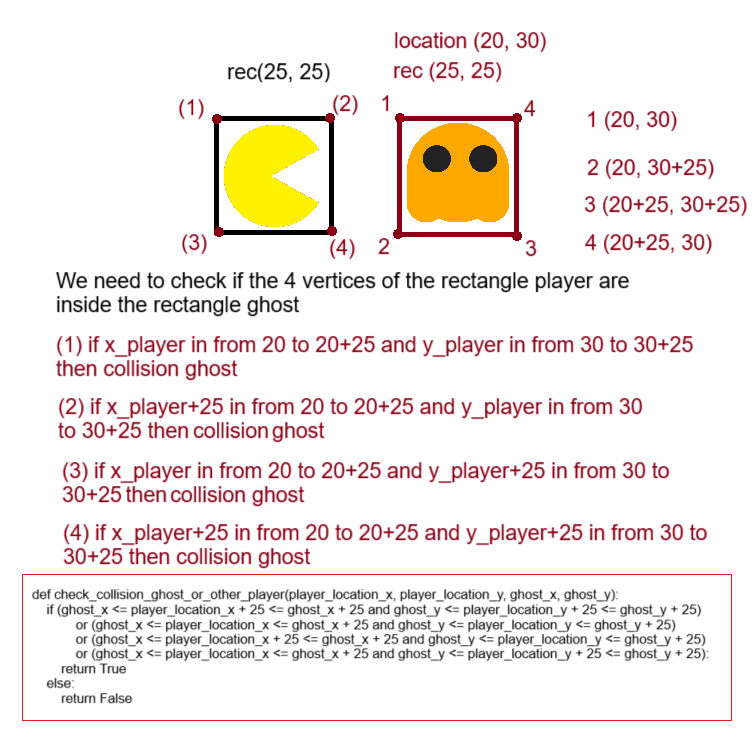
\includegraphics[width=15cm, height=18cm]{collision_ghost.png}
    \caption{Kiểm tra va chạm giữa người chơi và ma}
\end{figure}

\newpage
\subsubsection{Hàm xử lý va chạm với các con ma}
\begin{lstlisting}[language=Python]
def check_player_collisions_ghosts(player_location_x, player_location_y):
    global red_ghost_x, red_ghost_y, blue_ghost_x, blue_ghost_y, pink_ghost_x, pink_ghost_y, orange_ghost_x, \
        orange_ghost_y, red_ghost_dead, blue_ghost_dead, pink_ghost_dead, orange_ghost_dead
    player_dead = True
    eaten_ghosts = [False, False, False, False]  # red, blue, orange, pink
    # va chạm với ma
    collisions_red = check_collision_ghost_or_other_player(player_location_x, player_location_y, red_ghost_x,red_ghost_y)
    if collisions_red:
        if ghost_is_slow and not red_ghost_dead:
            red_ghost_y = len(map_level) // 2 * 25
            red_ghost_x = len(map_level[0]) // 2 * 25
            red_ghost_dead = True
            eaten_ghosts[0] = True
        else:
            return player_dead, eaten_ghosts
    collisions_blue = check_collision_ghost_or_other_player(player_location_x, player_location_y, blue_ghost_x,blue_ghost_y)
    if collisions_blue:
        if ghost_is_slow and not blue_ghost_dead:
            blue_ghost_y = (len(map_level) - 1) // 2 * 25
            blue_ghost_x = len(map_level[0]) // 2 * 25
            blue_ghost_dead = True
            eaten_ghosts[1] = True
        else:
            return player_dead, eaten_ghosts
    collisions_pink = check_collision_ghost_or_other_player(player_location_x, player_location_y, pink_ghost_x,pink_ghost_y)
    if collisions_pink:
        if ghost_is_slow and not pink_ghost_dead:
            pink_ghost_y = (len(map_level) - 2) // 2 * 25
            pink_ghost_x = (len(map_level[0]) - 1) // 2 * 25
            pink_ghost_dead = True
            eaten_ghosts[3] = True
        else:
            return player_dead, eaten_ghosts
    collisions_orange = check_collision_ghost_or_other_player(player_location_x, player_location_y, orange_ghost_x,orange_ghost_y)
    if collisions_orange:
        if ghost_is_slow and not orange_ghost_dead:
            orange_ghost_y = len(map_level) // 2 * 25
            orange_ghost_x = (len(map_level[0]) - 1) // 2 * 25
            orange_ghost_dead = True
            eaten_ghosts[2] = True
        else:
            return player_dead, eaten_ghosts

    return False, eaten_ghosts
\end{lstlisting}
Nếu ma đang bị làm chậm thì người chơi sẽ được tính là tiêu diệt con ma đó (con ma đó sẽ được đưa về chuồng) và được cộng điểm. Nếu con ma đó đang không bị làm chậm thì người chơi sẽ bị tính là mất mạng và bị trừ một nửa số điểm hiện có.


\subsubsection{Hàm xử lý va chạm giữa người chơi và người chơi}
\begin{lstlisting}[language=Python]
# ham va cham nguoi choi khac
def check_player_collisions_other_players(player_location_x, player_location_y, client, you_is_slowing):
    global thread_send_data_to_client
    score_increase = 0
    for key, value in data_clients.items():
        if client != key:
            # if slowing
            if value[9] and not you_is_slowing:
                result = check_collision_ghost_or_other_player(player_location_x, player_location_y, value[1], value[2])
                # and not flicker
                if result and not value[5]:
                    value[4] = True
                    value[6] //= 2
                    value[9] = False
                    # random player
                    x, y = random_empty_position(map_level)
                    value[1] = x
                    value[2] = y
                    # gửi lại dữ liệu cho các client
                    thread_send_data_to_client = threading.Thread(target=send_you_data, args=({"you": value},eval(key),))
                    thread_send_data_to_client.start()
                    score_increase += value[6]

    return score_increase

\end{lstlisting}
Nếu người chơi khác đang trong trạng thái không khỏe và bạn đang trong trạng thái khỏe mạnh thì khi đó bạn có thể tiêu diệt người chơi khác và cướp lấy một nửa số điểm của họ. 

\subsubsection{Hàm xử lý ăn thức ăn (viên gạch)}
\begin{lstlisting}[language=Python]
# hàm kiểm tra ăn thức ăn
def check_eat_food(player_location_x, player_location_y):
    global ghost_is_slow, ghost_slow_speed, ghost_speeds, ghost_slow_time_count
    total_new_score = 0
    eaten_food = False
    eaten_big_food = False
    # lấy điểm giữa của pacman
    center_player_x = player_location_x + 12
    center_player_y = player_location_y + 13
    # lấy kích thước 1 ô
    height_a_rec = HEIGHT_PLAYING // len(map_level)
    width_a_rec = WIDTH_PLAYING // len(map_level[0])
    if map_level[center_player_y // height_a_rec][center_player_x // width_a_rec] == 1:
        map_level[center_player_y // height_a_rec][center_player_x // width_a_rec] = 0
        total_new_score += 100
        eaten_food = True
    if map_level[center_player_y // height_a_rec][center_player_x // width_a_rec] == 2:
        map_level[center_player_y // height_a_rec][center_player_x // width_a_rec] = 0
        total_new_score += 500
        eaten_food = True
        ghost_is_slow = True
        eaten_big_food = True
        ghost_speeds = ghost_slow_speed
        ghost_slow_time_count += ghost_slow_time_default
    return eaten_food, total_new_score, eaten_big_food
\end{lstlisting}
Dựa vào vị trí để biết có hay không việc chạm vào 1 cục thức ăn, nếu mà cục thức ăn đó là cục thức ăn lớn thì các con ma sẽ bị làm chậm và các người chơi khác sẽ rơi vào trạng thái nguy hiểm.


\subsubsection{Hàm xử lý dữ liệu bảng điểm của người chơi}
\begin{lstlisting}[language=Python]
def run_handel_score_player():
    while running_handle_score:
        pygame.time.delay(delay_handle_score)
        if len(data_clients) > 0:
            data_score_players = {}
            for client_data in list(data_clients.values()):
                data_score_players[client_data[0]] = client_data[6]
            try:
                sorted_score_table = dict(sorted(data_score_players.items(), key=lambda item: item[1], reverse=True))
                first_seven_items = list(sorted_score_table.items())[:7]
                for client in connected_clients:
                    server_socket.sendto(json.dumps({"score_table": dict(first_seven_items)}).encode(), client)
            except:
                pass
# luong gui bang xep hang
send_data_score_to_all_client_thread = threading.Thread(target=run_handel_score_player)
send_data_score_to_all_client_thread.start()
\end{lstlisting}
Cứ mỗi nửa giây sẽ tổng hợp điểm của người chơi và gửi về cho các client 7 người có điểm số cao nhẩt được xếp theo thứ tự giảm dần. Công việc này được thực hiện ở một luồng riêng biệt để có thể gửi dữ liệu liên tục đến các client mà không ảnh hưởng điến việc xử lý khác.

\subsubsection{Hàm xử lý sinh thêm thức ăn mới sau mỗi 30 giây}
\begin{lstlisting}[language=Python]
def run_auto_produce_food():
    while running_produce_food:
        pygame.time.delay(delay_auto_produce_food)
        global map_level
        if count_numbers(map_level, 1) < 50:
            # số lượng thức ăn nhỏ
            map_level = random_to_number(map_level, 30)
        if count_numbers(map_level, 2) < 3:
            # số lượng thức ăn lớn
            map_level = random_to_number(map_level, 2, 2)
# luong randon food
thread_random_food = threading.Thread(target=run_auto_produce_food)
thread_random_food.start()
\end{lstlisting}
Thực hiện bổ sung thức ăn sau mỗi 30 giây trên bản đồ nếu thức ăn đã bị người chơi ăn còn ít hơn số lượng định sẵn.


\subsubsection{Các hàm phục vụ việc random thức ăn và vị trí người chơi}
\begin{lstlisting}[language=Python]
# ramdom food
def random_to_number(matrix, num_to_replace=10, replace_to=1):
    n = len(matrix)  # Số hàng của ma trận
    m = len(matrix[0])  # Số cột của ma trận

    # Tìm và chọn ngẫu nhiên các vị trí 0 để thay thế
    replace_indices = []
    for _ in range(num_to_replace):
        while True:
            i = random.randint(0, n - 1)  # Chọn một chỉ số hàng ngẫu nhiên
            j = random.randint(0, m - 1)  # Chọn một chỉ số cột ngẫu nhiên
            if matrix[i][j] == 0:  # Nếu giá trị tại vị trí này là 0, thì thêm vào danh sách và thoát vòng lặp
                replace_indices.append((i, j))
                break

    # Thay thế các số 0 tại các vị trí đã chọn thành 1
    for i, j in replace_indices:
        matrix[i][j] = replace_to

    return matrix


# tìm vị trí trống trong matrix map
def random_empty_position_in_map(matrix):
    empty_positions = [(y, x) for y in range(len(matrix) - 1) for x in range(len(matrix[0]) - 1) if matrix[y][x] == 0]
    if empty_positions:
        return random.choice(empty_positions)
    else:
        return None


# random và tính toán vị trí trống
def random_empty_position(matrix):
    y, x = random_empty_position_in_map(matrix)
    return x * 25, y * 25

\end{lstlisting}


%%%%%%%%%%%%%%%%%%%%%%%%%%%%%%%%%
\section{Thực Thi}

Trong phần này, chúng tôi sẽ hướng dẫn các bước khi chạy trò chơi Pacman đa người chơi và mô tả các chức năng có trong game.

\subsection{Triển Khai Mã Nguồn}

Đầu tiên, hãy chắc chắn rằng bạn đã cài đặt Python và thư viện Pygame trên máy tính của mình. Sau đó, tải mã nguồn của trò chơi Pacman từ kho lưu trữ Git.

\subsubsection{Kiểm tra Python có sẵn hay không}
\begin{lstlisting}[language=bash]
$ python3 --version
\end{lstlisting}

\subsubsection{Cài đặt Python}
\begin{lstlisting}[language=bash]
$ sudo apt update
$ sudo apt install python3
\end{lstlisting}

\subsubsection{Cài đặt thư viện Pygame}
\begin{lstlisting}[language=bash]
$ pip install pygame
\end{lstlisting}

\subsubsection{Tải mã nguồn từ github}
\begin{lstlisting}[language=bash]
$ git clone https://github.com/dolehuy00/PacmanGameWithSocket.git
\end{lstlisting}


\subsection{Khởi động Trò Chơi}

Mở Terminal và di chuyển đến thư mục chứa mã nguồn của trò chơi. Chạy lệnh để khởi động trò chơi Pacman.
\subsubsection{Chạy server}
\begin{lstlisting}[language=bash]
$ python server_data_udp.py
$ python server_chat_tcp.py
\end{lstlisting}

\subsubsection{Chạy client}
\begin{lstlisting}[language=bash]
$ python client_1.py
\end{lstlisting}

\subsection{Chơi Trò Chơi}

Sau khi trò chơi khởi động, màn hình chờ sẽ được hiển thị, tại đây bạn có thể nhập tên của mình trước khi vào phòng. Sau đó bạn có thể nhấn enter hoặc nút "Start" để bắt đầu vào phòng chơi.

Trong quá trình chơi trò chơi Pacman, có một số tình huống xảy ra như sau:

\begin{enumerate}
    \item \textbf{Pacman Ăn Một Viên Gạch:} Khi Pacman đi qua một viên gạch, viên gạch sẽ biến mất và người chơi sẽ nhận được điểm số tương ứng.
    \item \textbf{Pacman Tiếp Xúc Với Ma:} Nếu Pacman tiếp xúc với một con ma, có thể xảy ra:
        \begin{itemize}
            \item Nếu ma đang ở trạng thái làm chậm (sau khi bạn ăn được viên gạch lớn), Pacman sẽ ăn được ma và ma sẽ được đưa về chuồng giữa bản đồ, bạn sẽ được cộng điểm.
            \item Nếu ma không ở trạng thái làm chậm, Pacman sẽ bị mất mạng và được dịch chuyển đến vị trí ngẫu nhiên, đồng thời mất nửa số điểm hiện có.
        \end{itemize}
     \item \textbf{Pacman Tiếp Xúc Với Người Chơi Khác:} Nếu Pacman tiếp xúc với một người chơi khác, có thể xảy ra:
        \begin{itemize}
            \item Nếu người chơi khác đang đang ở trạng thái suy yếu (có màu xanh) (sau khi bạn ăn được viên gạch lớn), bạn sẽ tiêu diệt được người chơi khác, họ sẽ bị đưa đi vị trí ngẫu nhiên, bạn sẽ cướp được nửa số điểm của họ.
            \item Nếu người chơi khác không ở trạng thái suy yếu hoặc cả 2 đểu bị suy yếu, thì không có việc gì xảy ra cả.
        \end{itemize}    
    \item \textbf{Pacman ăn viên gạch năng lượng(thức ăn lớn):} Khi Pacman ăn một viên gạch năng lượng, nó sẽ trở thành "siêu phẩm" trong một khoảng thời gian ngắn, có khả năng ăn được các con ma mà không bị tấn công và làm suy yếu các người chơi khác.
    \item \textbf{Ăn Hết Các Viên Gạch:} Nếu Pacman ăn hết tất cả các viên gạch trên màn hình, trong khoảng 30 giây tiếp theo trò chơi sẽ tự động sinh ra các viên gạch mới và người chơi có thể đoạt được các viên gạch lớn để tối ưu số điểm của mình.
\end{enumerate}
\newpage
%%%%%%%%%%%%%%%%%%%%%%%%%%%%%%%%%
\section{Kết Luận}
Đường dẫn đến dự án trên github: \href{https://github.com/dolehuy00/PacmanGameWithSocket.git}{https://github.com/dolehuy00/PacmanGameWithSocket.git}
Đường dẫn đến trang web: \href{https://dolehuy00.github.io/PacmanGameWithSocket/}{https://dolehuy00.github.io/PacmanGameWithSocket/}


Kết quả đạt được:
\begin{itemize}
    \item Biết được cách sử dụng thư viện pygame để tạo ra game đơn giản.
    \item Biết các sử dụng socket để gửi dữ liệu thông qua mạng máy tính trong localhost.
    \item Cải tiến game cổ điển offline thành có thể chơi được nhiều người.
\end{itemize}
Tổng kết: Việc phát triển ứng dụng game đã mang lại thêm nhiều kinh nghiệm trong lập trình với ngôn ngữ Python, cú pháp và cách xử lý dữ liệu.
\end{document}

